\documentclass[main.tex]{subfiles}

\begin{document}

\section{Besoins du projet}

\subsection{Contexte}

\begin{figure}[htpb]
	\centering
	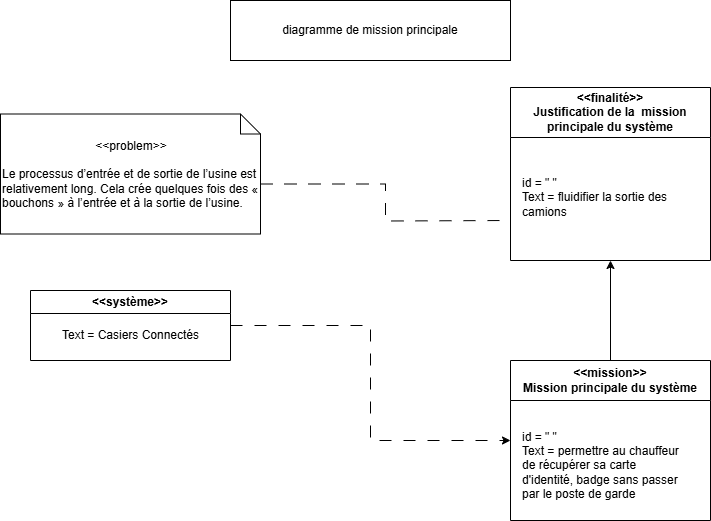
\includegraphics[width=1\textwidth]{../images/Diagramme_de_mission_principale.drawio.drawio}
	\caption{Diagramme de mission principale}
	\label{fig:DDMP}
\end{figure}

\quad Le projet Casiers RFID Motorisés est développé pour l’entreprise Sylvamo France SA, située à Saillat-sur-Vienne. Sylvamo est un acteur majeur dans la production de papier, employant environ 600 personnes sur son site en France. L’usine fonctionne sous des normes strictes de sécurité et de certification, ce qui impose des contraintes spécifiques à la gestion des accès et des flux logistiques.

L’un des enjeux majeurs de l’usine est la gestion des entrées et sorties des chauffeurs routiers qui livrent quotidiennement des matières premières. Actuellement, ces chauffeurs doivent déposer leur pièce d’identité à l’entrée et ont en échange un badge pour circuler sur le site. Lors de leur départ, un agent de sécurité leur restitue leur document après vérification du badge. Ce processus, bien que sécuritaire, engendre bien des ralentissements et des files d’attente importantes, notamment lorsque les conducteurs étrangers qui ne parlent pas français ou anglais.

Le projet vise à automatiser cette gestion à l’aide d’un système de casiers motorisés couplé à un contrôle RFID. Lorsqu’un chauffeur entre sur le site, son badge RFID sera associé à un casier sécurisé contenant son document d’identité. À la sortie, en déposant son badge RFID dans un lecteur, le système ouvrira automatiquement le casier correspondant, réduisant ainsi le temps d’attente et fluidifiant le trafic des camions.

En plus de cet avantage logistique, l’utilisation des badges RFID permettra également un suivi numérique des chauffeurs (heure d’entrée, points de passage, heure de sortie), avec stockage des données dans une base de données SQL pour une possible exploitation statistique ultérieure.

Le projet est développé par trois étudiants dans le cadre d’un BTS CIEL (Cybersécurité, Informatique et Électronique) au Lycée Turgot de Limoges. Sa réalisation est prévue de janvier 2025 à mai 2025, avec un budget alloué de 1000 €.


\subsection{Introduction}

\quad Dans le cadre de notre formation en BTS CIEL (Cybersécurité Informatique et Réseaux Électroniques option A Réseaux Informatiques), nous avons été amenés à concevoir un projet technologique répondant à une problématique réelle d’entreprise. Le projet retenu porte sur la mise en place d’un système de casiers RFID motorisés pour fluidifier la gestion des documents d’identité des chauffeurs à l’entrée et à la sortie du site industriel Sylvamo.

L’objectif principal est de développer une solution automatisée et sécurisée permettant d’associer un badge RFID à un casier contenant les papiers du chauffeur. Grâce à un système de lecture RFID et une interface logicielle dédiée, l’agent de sécurité pourra facilement déposer et restituer les documents, réduisant ainsi le temps d’attente à la sortie de l’usine.

Ce projet mobilise différentes technologies et compétences, notamment :

\begin{itemize}
   \item La programmation en C++ et C\# pour le développement du logiciel de gestion
   \item L’intégration d’une base de données MariaDB pour le stockage et le suivi des informations
   \item L’utilisation de servomoteurs et de DEL RGB pour la gestion physique des casiers
   \item Un réseau sécurisé avec un pare-feu logiciel pour protéger l’ensemble du système
\end{itemize}

La réalisation du projet s’effectuera en plusieurs étapes, de la conception initiale jusqu’à l’intégration et les tests, afin de garantir une solution fonctionnelle et adaptée aux besoins du site industriel.

\newpage

\end{document}
